\documentclass[]{article}

%opening
\title{Considerations regarding the feasibility of an sklearn-based RNAz implementation}
\author{Christopher}
\usepackage{graphicx}
\usepackage{float}
\usepackage{subcaption}
\captionsetup[subfigure]{list=true, font=small, labelfont=bf, 
	labelformat=brace, position=top}

\begin{document}
\maketitle

\section{Introduction}

As has been discussed before, there are indicators that LibSVM is no longer an optimal solution for an efficient implementation of a binary SVM classifier. Reasons discussed till this point include a potential run time inefficiency, less up to date code and the undeniable problematic of having to implement bindings across multiple programming languages for full functionality. This short report gives an overview of first experimental results using a very rudimentary sklearn SVM implementation and potential next steps. 

\section{Experimental results}

A simple parser and interface to create Svhip-compatibility for sklearn was implemented in Python. Functionality at this point include the loading of Svhip-generated processed data for training, a hyper parameter optimization modeled after the grid search used by Svhip and the possibility to save a trained classifier as a binary file (not natively supported by sklearn). The rudimentary program has been added to the corresponding Github repository. For a first test, a well-established data set generated with Svhip was used to train an sklearn classifier. The data set included data from 30 Rfam families and consisted of 7772 training instances in total. Using the sklearn interface, a classifier was trained and used to predict the original RNAz 2.0 test set for reference. Figure 1 visualizes the performance on this set.  A simple grid search with 400 value pairs in total was used for hyper parameter optimization. \newline

\begin{figure}[H]
	\centering
	\begin{subfigure}[b]{0.45\textwidth}
		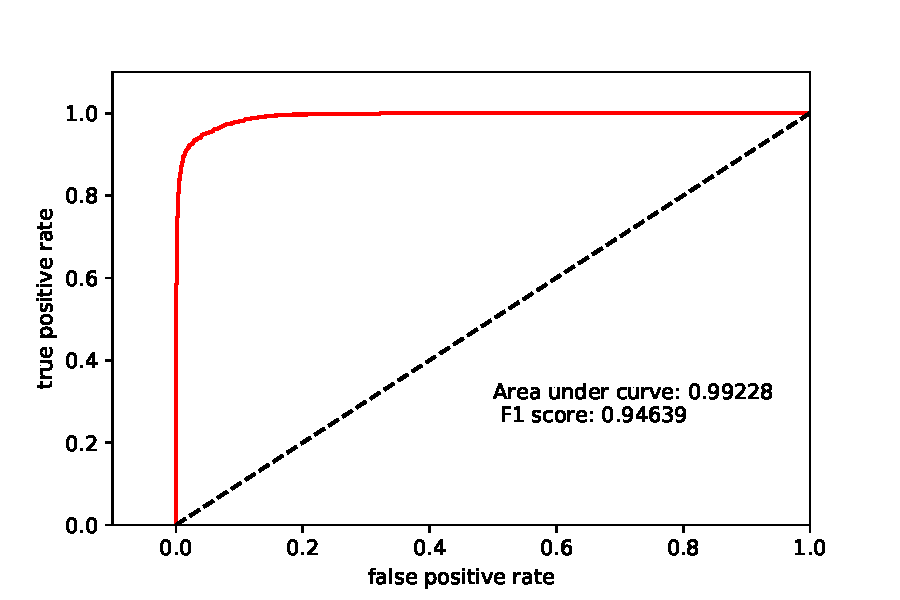
\includegraphics[width=1\textwidth]{example_sklearn.pdf}
		\caption{}
		\label{fig1}
	\end{subfigure}
	\hfill
	\begin{subfigure}[b]{0.42\textwidth}
		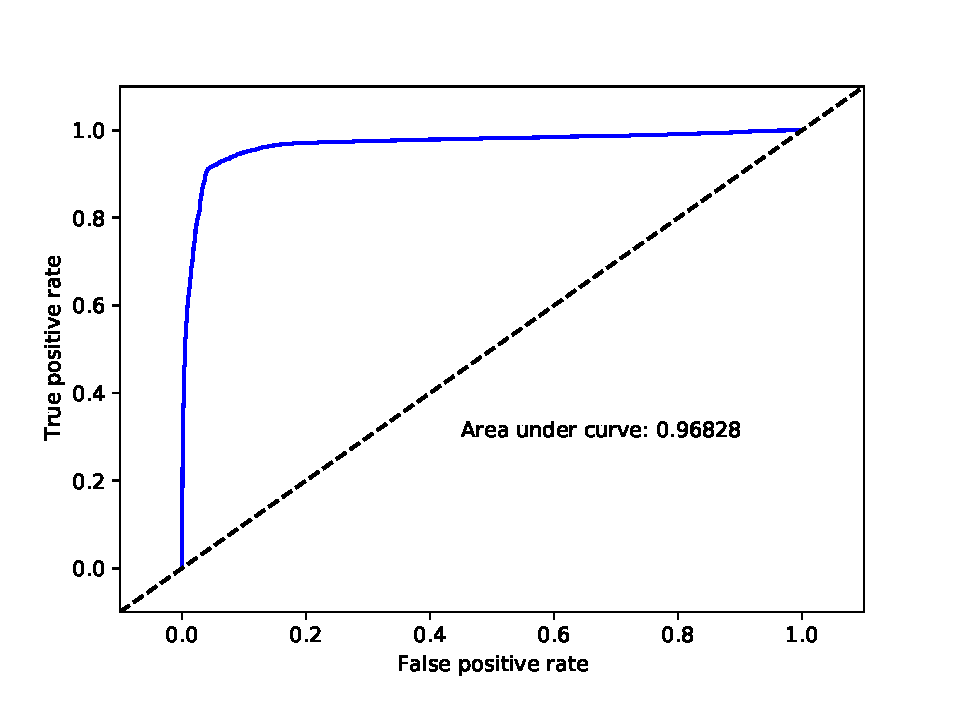
\includegraphics[width=1\textwidth]{libsvm_example.pdf}
		\caption{}
		\label{fig1}
	\end{subfigure}
	\caption{Comparison of SVM classifier performance using the sklearn implementaion (a) and LibSVM (b). For both classifiers, the identical training set with 7772 training instances and the unmodified RNAz 2.0 test set were used. }
\end{figure}

As can be observed, the sklearn trained classifier outcompetes the standard LibSVM trained classifier by a margin of almost 3\%. Given the vulnerability of SVM based classification on large data sets to false positives, this increase should be considered significant. In fact, the accuracy is now practically identical to the performance of the unmodified RNAz 2.0 classifier (difference of 0.11\%). Also, the run time for parameter optimization and classifier training is with 217 s several orders of magnitude lower than with the standard LibSVM implementation. It can however be assumed, that the slower performance of the LibSVM might in part be caused by inefficient Python bindings of this library. This is nonetheless an issue of high significance when attempting to streamline the classifier retraining process. 

\section{Issues \& Discussion}

As was shown with this first example, sklearn is in terms of accuracy and run time performance a more than viable alternative to the LibSVM library. There are however some remaining issues when considering a reimplementation of the RNAz core framework. \newline

First off, RNAz utilizes multiple helper scripts (rnazWindow.pl and others) written in Perl to support data preparation and filtering. Since these are mostly detached from the program core implemented in C (that is to say, they are also not dependent on any LibSVM-bindings) and perform very efficiently as they are, I would strongly argue for leaving these in their current state. \newline
The core program itself is loosely separable in feature vector calculation based on input data and the classifier-handler. The latter could be trivially ported to Python and the sklearn interface. The former introduces the problem of using a LibSVM-backed support vector regression for estimating the z-score of minimum free energy. Porting this functionality is non-trivial as a complete retraining of the SVR would be necessary in any case. \newline 

Lastly, an obvious drawback is that there appears to be no sideway compatibility between LibSVM and sklearn, i.e. it is currently impossible to migrate the current RNAz 2.0 classifier into the sklearn implementation without loss. A retraining also is not possible, as the original training set is unavailable. 

\section{Conclusion}

In sum, while it would certainly be beneficial from an efficiency point of view to attempt the port of RNAz to Python and the sklearn library, there are issues that would require additional time to solve, most importantly the inevitable retraining of the SVR for z-score of MFE approximation. It is advantageous that not the entire RNAz code would have to be ported to support sklearn, as a significant part of the program is modularized and independent of the core program. Also, this report has shown that the Svhip retraining pipeline works very efficiently with sklearn almost out of the box, given the additional interface presented here.  

\end{document}